\appendix
\def\thesection{S\arabic{section}}
\def\thesubsection{S\arabic{section}.\arabic{subsection}}
\setcounter{equation}{0}
\renewcommand{\theequation}{S\arabic{equation}}
\setcounter{page}{1}

\begin{center}
    {\LARGE Tail risk in the tail: Estimating high quantiles when a related variable is extreme\\
  \bf Supplementary Material\\
  }
\end{center}


\section{Parametric models for the tail dependence function}\label{sS3}
In this section, we provide tail dependence functions for four parametric models considered in simulation studies and the application. 
\begin{enumerate}[label=(\arabic*)]
    \item The bivariate logistic distribution function with standard Fr\'echet margins is given by
    $$G(x,y;\theta) = \exp\left\{-(x^{-1/\theta}+y^{-1/\theta})^\theta\right\},$$
    where $x, y>0$ and $\theta \in (0,1]$. The upper tail dependence function in this case has the form
\begin{equation}\label{tail_log}
R(x,y;\theta) = x + y - (x^{1/\theta}+y^{1/\theta})^{\theta}.
\end{equation}
    
    \item The bivariate H\"{u}sler-Reiss distribution function with standard Fr\'echet margins is
    $$G(x,y;\theta) = \exp\left\{-x^{-1}\Phi\Bigl(\theta^{-1}+\frac{\theta}{2}\log(y/x)\Bigr)-y^{-1}\Phi\Bigl(\theta^{-1}+\frac{\theta}{2}\log(x/y)\Bigr)\right\},$$
    where $x, y>0$, $\theta >0$ and $\Phi(\cdot)$ is the standard normal distribution function. Its tail dependence function is given by
\begin{equation}\label{tail_hr}
R(x,y;\theta) = x + y - x\Phi\Bigl(\theta^{-1}+\frac{\theta}{2}\log(x/y)\Bigr)-y\Phi\Bigl(\theta^{-1}+\frac{\theta}{2}\log(y/x)\Bigr).
\end{equation}


    \item The bivariate asymmetric logistic distribution with standard Fr\'echet margins has distribution function of the form
$$
 G(x,y;\psi_1,\psi_2,\theta) = \exp\Bigl\{-(1-\psi_1)/x-(1-\psi_2)/y- \bigl((\psi_1/x)^{1/\theta}+(\psi_2/y)^{1/\theta}\bigr)^\theta\Bigr\},
$$
where $x,y>0$, $\theta\in(0,1]$ and $\psi_1,\psi_2\in [0,1]$. Its tail dependence function is given by
\begin{equation}\label{tail_alog}
R(x,y;\psi_1,\psi_2,\theta)=\psi_1x+\psi_2y-\bigl((x\psi_1)^{1/\theta}+(y\psi_2)^{1/\theta}\bigr)^{\theta}.
\end{equation}
    
    \item The joint density function of a standard bivariate $t$ distribution with $\n>0$ degrees of freedom and correlation parameter $\r\in(-1,1)$ is written as
$$
 f_{T}(\wb;\rho,\nu) = \dfrac{\Gamma\bigl((\nu+2)/2\bigr)}{\sqrt{1-\rho^2}\nu\pi\Gamma(\nu/2)}\Bigl(1+\dfrac{1}{\nu}\wb^T\Omega^{-1}\wb\Bigr)^{-(\nu+2)/2},\quad \Omega=\bma 1 & \r\\ \r & 1 \ema,\quad \wb\in\rbb^2.
 $$
For $\r\in(0,1)$, its upper tail dependence function is given by
\begin{equation}\label{tail_t}R(x,y;\rho,\nu)=xF_{T}\Bigl(\sqrt{\frac{\nu+1}{1-\rho^2}}\bigl(\rho-(y/x)^{-1/\nu}\bigr);\nu+1 \Bigr)+yF_{T}\Bigl(\sqrt{\frac{\nu+1}{1-\rho^2}}\bigl(\rho-(x/y)^{-1/\nu}\bigr);\nu+1 \Bigr), 
\end{equation}
where $F_T(\cdot;\n)$ is the distribution function of the standard Student $t$ distribution with $\n$ degrees of freedom. Expression~\eqref{tail_t} is founded following \cite{DemartaMcNeil2005}, where the lower tail dependence function of the bivariate $t$ distribution is given.

\end{enumerate}

\section{Plots of \texorpdfstring{$R(1,\h)$}{R1eta} as a function of \texorpdfstring{$\h$}{eta}}
\label{sup:tail_fun}

Figure~\ref{tail_fun} illustrates function  $R(1,\h)$ under the four tail dependence models listed in Section~\ref{sS3} and used in simulation studies and the application. The upper bound $R(1,\h)\le \h$ for $\h\in(0,1)$ corresponds to the case of complete positive dependence. This implies that when tail dependence is fairly strong, $R(1,\h)$ is close to the linear function $R(1,\h)=\h$. For a given $p$, $\h^*$ in $R(1,\eta^*) = p$ decreases as tail dependence gets stronger. 

\begin{figure}[ht]
  \centering 
  \subfigure[Logistic]{
    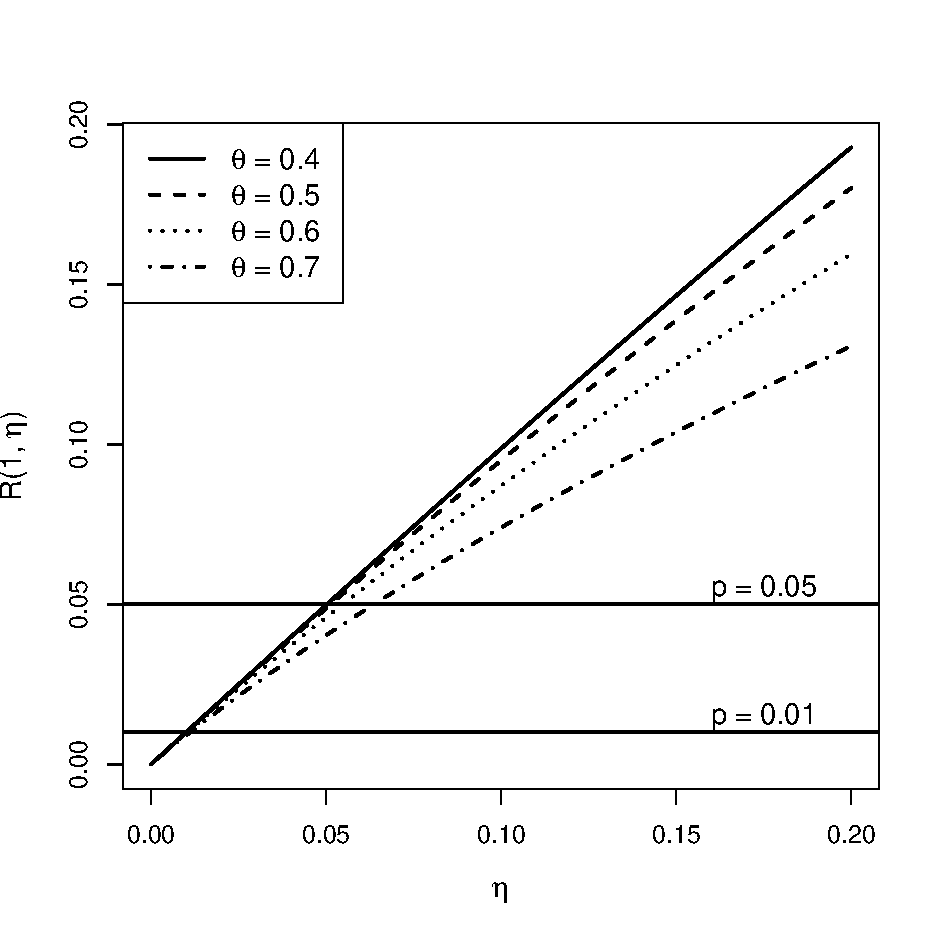
\includegraphics[width=0.3\linewidth]{tailfun_log.pdf}}
  \subfigure[H\"{u}sler-Reiss]{
    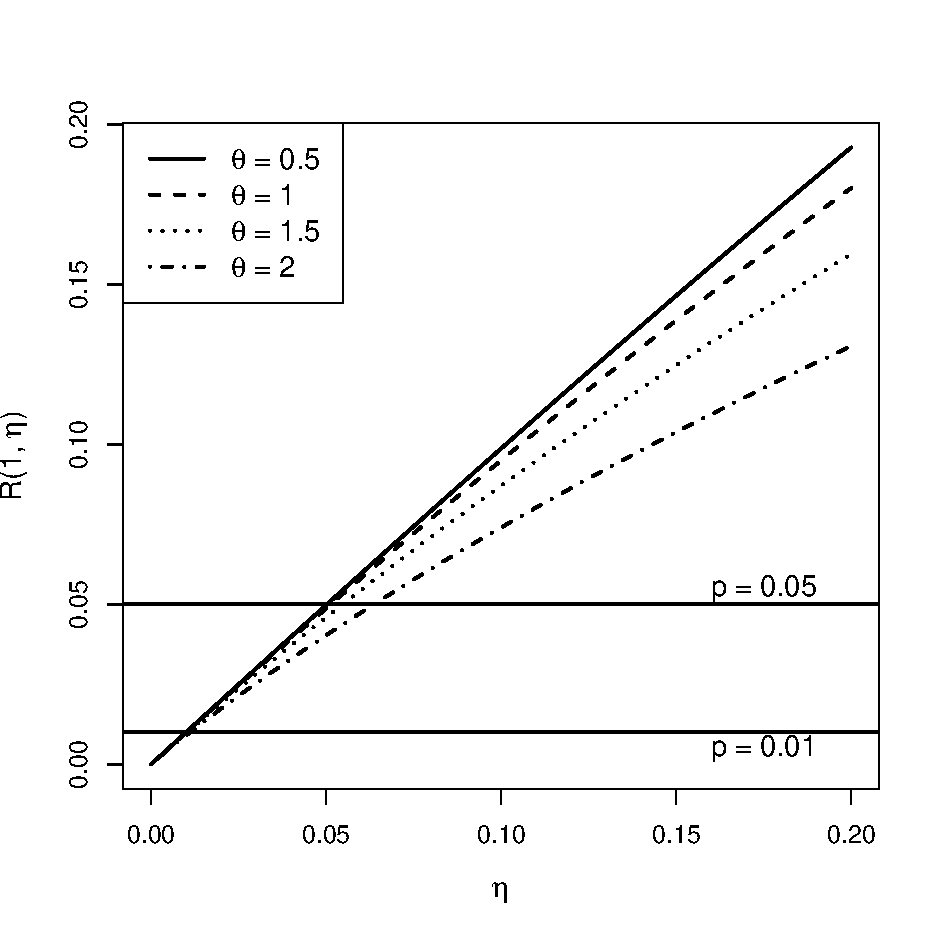
\includegraphics[width=0.3\linewidth]{tailfun_hr.pdf}}
    \subfigure[Asymmetric logistic]{
    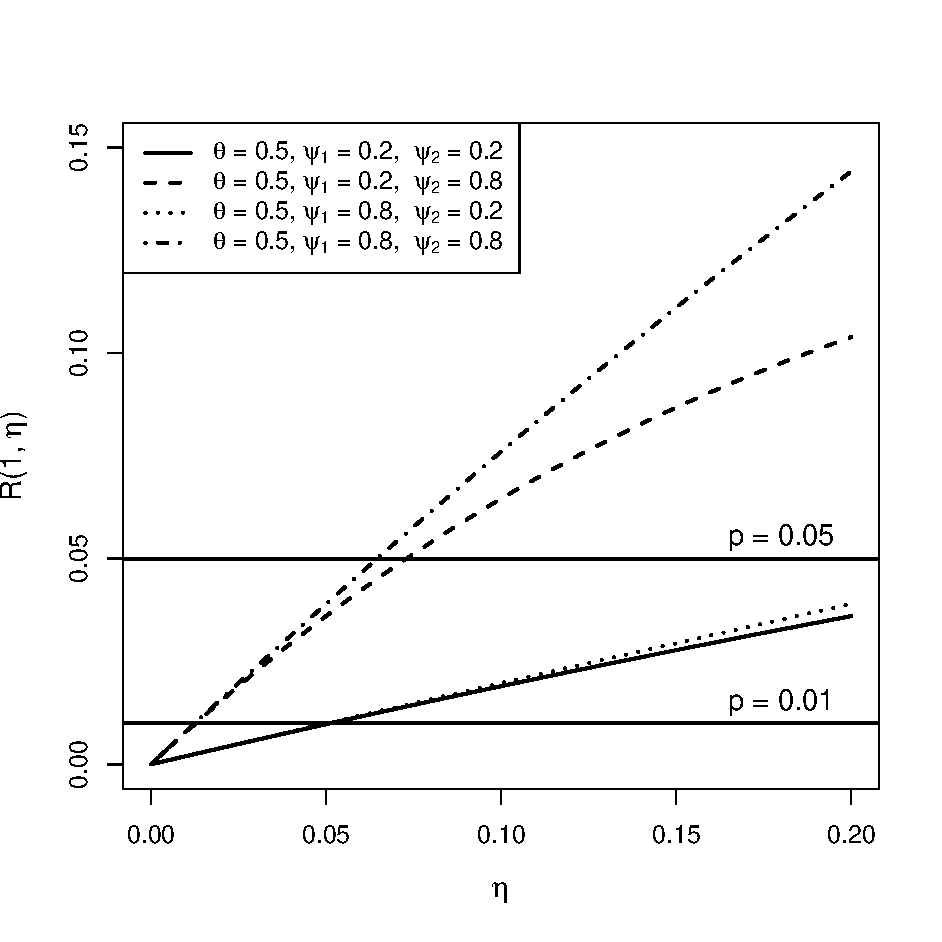
\includegraphics[width=0.3\linewidth]{tailfun_alog.pdf}}
    \subfigure[Bivariate t]{
    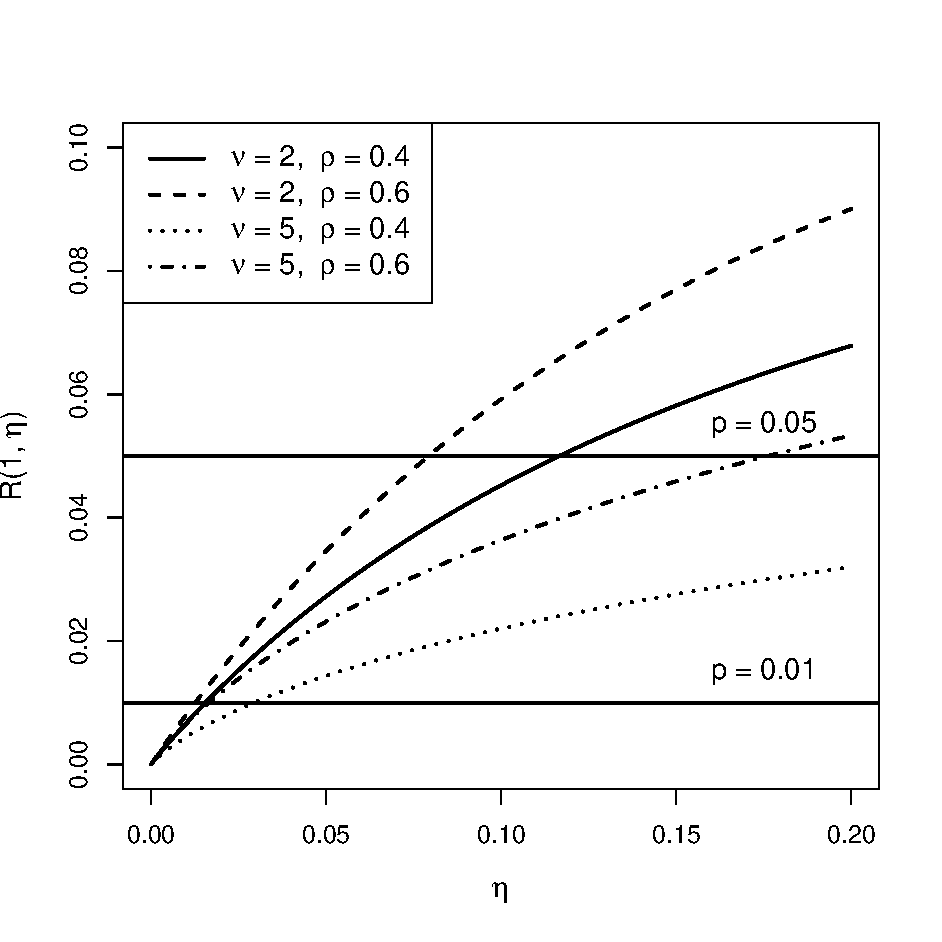
\includegraphics[width=0.3\linewidth]{tailfun_t.pdf}}
    \caption{Plots of $R(1,\eta)$ as a function of $\eta$ under various tail dependence models.}
  \label{tail_fun}
\end{figure}

\clearpage

\section{Two-stage procedure for estimating \texorpdfstring{$\CoVaR_{t}^{s|i}(p_2|p_1)$}{CoVaRt}}\label{sS4}

To estimate CoVaR dynamically, we need to apply a two-stage procedure, which can be summarized in the steps below.

\noindent{\bf Step 1 }(Univariate GARCH model estimation): Assume that $\{X_t^i\}_{t\in \nbb}$ and $\{X_t^s\}_{t\in \nbb}$ each follows an AR(1)-GARCH(1,1) process \citep{Bollerslev1986} satisfying the following model equations:
\begin{align*}
&X_t^{i} = \mu_t^{i} + \sigma_t^{i}Z_t^{i}, \quad \mu_t^{i} = \alpha_0^{i} + \alpha_1^{i}X_{t-1}^{i}, \quad (\sigma_t^{i})^2 = \beta_0^{i} + \beta_1^{i}(\sigma_{t-1}^{i}Z_{t-1}^{i})^2 + \beta_2^{i}(\sigma_{t-1}^{i})^2,\\
&X_t^{s} = \mu_t^{s} + \sigma_t^{s}Z_t^{s}, \quad \mu_t^{s} = \alpha_0^{s} + \alpha_1^{s}X_{t-1}^{s}, \quad (\sigma_t^{s})^2 = \beta_0^{s} + \beta_1^{s}(\sigma_{t-1}^{s}Z_{t-1}^{s})^2 + \beta_2^{s}(\sigma_{t-1}^{s})^2,
\end{align*}
where sequences of innovations $\{Z_t^{i}\}_{t\in \nbb}$ and $\{Z_t^{s}\}_{t\in \nbb}$ are  i.i.d. with zero mean and unit variance. Parameters of the AR(1)-GARCH(1,1) filters are estimated using maximum likelihood assuming a standardized skew-$t$ distribution (\cite{FernandezSteel1998}) for the innovations. With the estimates of conditional means and volatilities, we can obtain two sequences that could be used as proxies for realized innovations: 
\begin{equation}
\label{inno}
    \bigl\{\hat{Z}_t^{i} = (X_t^{i} - \hat{\mu}_t^{i})/{\hat{\sigma}_t^{i}}\bigr\},\qquad \bigl\{\hat{Z}_t^{s} = (X_t^{s} - \hat{\mu}_t^{s})/{\hat{\sigma}_t^{s}}\bigr\}.
\end{equation}

\noindent{\bf Step 2 }(Dynamic CoVaR estimation): Based on the time series representation of losses, $\CoVaR_{t}^{s|i}(p_2|p_1)$ can be expressed as
\begin{align*}
1 - p_2  &= \pbb\bigl(X_t^s \geq \CoVaR_{t}^{s|i}(p_2|p_1) | X_t^i\geq \VaR^i_{t}(p_1);\ \FC_{t-1}^i,\   \FC_{t-1}^s\bigr)\\
&=\pbb\Bigg(Z_t^s \geq \dfrac{\CoVaR_{t}^{s|i}(p_2|p_1)-\m_t^s}{\s_t^s}\Big | Z_t^i\geq \dfrac{\VaR^i_{t}(p_1)-\m_t^i}{\s_t^i};\ \FC_{t-1}^i,\   \FC_{t-1}^s\Biggr).
\end{align*}
This suggests first estimating risk measures based on the samples of realized innovations in \eqref{inno}, treated as i.i.d., and then computing the dynamic forecasts for time $t$ via
\begin{equation}
\widehat{\CoVaR}_{t}^{s|i}(p_2|p_1) = \hat{\mu}_t^{s} + \hat{\s}_t^s \widehat{\CoVaR}_{Z^s|Z^i}(p_2|p_1),\qquad \widehat{\VaR}^i_{t}(p_1)=\hat{\mu}_t^i + \hat{\s}_t^i\widehat{\VaR}_{Z^i}(p_1).
\end{equation}

The two-step procedure is theoretically justified as follows. First, as shown in \cite{Hoga2019_sup} (Proposition 2 in Appendix A), under the assumption that the estimation model is correctly specified, the tail empirical process based on the estimated innovations is arbitrarily close to that based on the true innovations. The difference is so small that it does not interfere with the asymptotic behavior of the latter process. This result holds for both series. Second, the results above immediately lead to the conclusion that the bivariate tail empirical process based on the two estimated innovations is arbitrarily close to that based on the two true innovations, because the difference is bounded by the sum of the differences in the two marginals. This is an obvious result due to the fact that two indicators of a joint event based on the estimated and true innovation can differ only if at least one pair of marginal indicators differs. In other words, we can show that the bivariate tail empirical process based on the two estimated innovations share the same asymptotic behavior as that based on two true innovations, which has
a bivariate Gaussian process as the limit. Such a result is the starting point for proving the asymptotic behavior of the moment estimator as in \cite{Einmahl_etal2012_sup}. Therefore, in the third step, following the lines of the proof in \cite{Einmahl_etal2012_sup}, we obtain the same asymptotic result for the moment estimator with the same speed of convergence. Fourth, we can get the asymptotic behavior of all other components needed in the proof of Theorem \ref{main_theorem_asymptotic_normality} following from the marginal tail empirical process results. Finally, combining all components and again following the proof of Theorem \ref{main_theorem_asymptotic_normality}, one can show the asymptotic normality of the estimator for the time varying CoVaR.

This strategy of proof follows similar ideas for other estimators in the literature. For instance, \cite{Hoga2022} provides an extension to situations where filtering is based on a general location-scale model. See also \cite{Girard_etal2021} for results on residual-based extreme value estimators in heavy-tailed regression models.


We note that in Step~1 above, if there is evidence of time changing correlation structure in the data, an alternative is to use a bivariate GARCH filter as was previously done in \cite{Girardi2013_sup} and \cite{NoldeZhang2018_sup}. For the data considered here, filtering out correlation led to weaker tail dependence potentially invalidating the assumption of tail dependence (for example, see Figure~\ref{sc_dcc}). We, therefore, chose to apply the GARCH filters only marginally.  

\begin{figure}[ht]
  \centering
  \subfigure{
  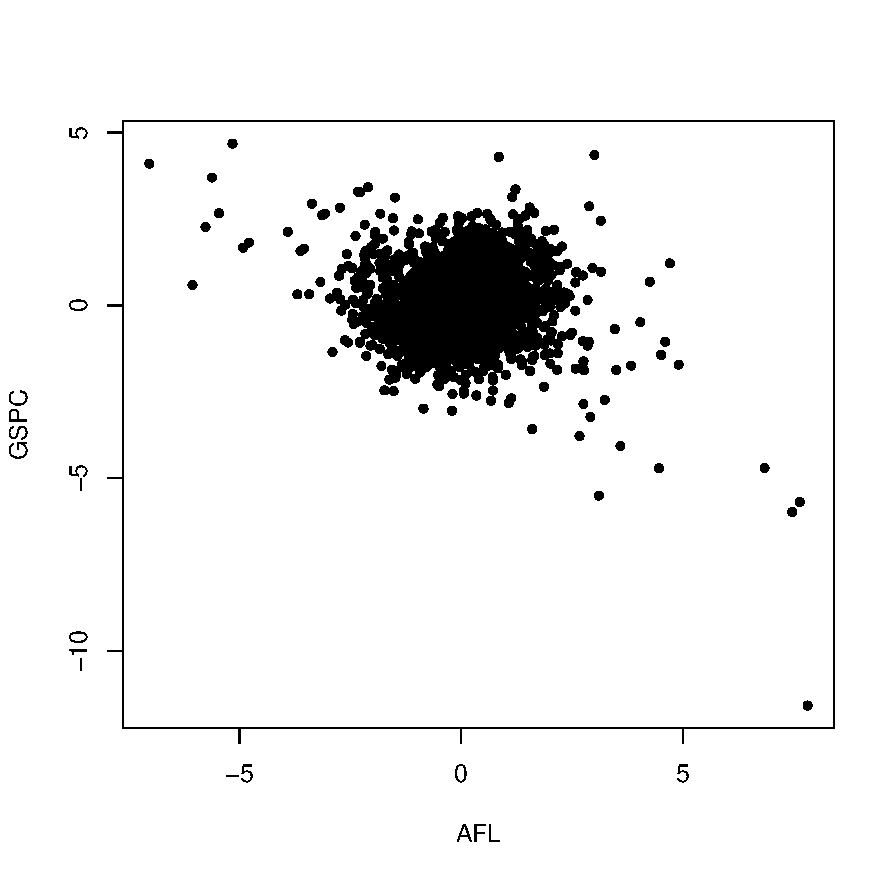
\includegraphics[width=0.4\linewidth]{scplot_AFL.pdf}}
  \subfigure{
  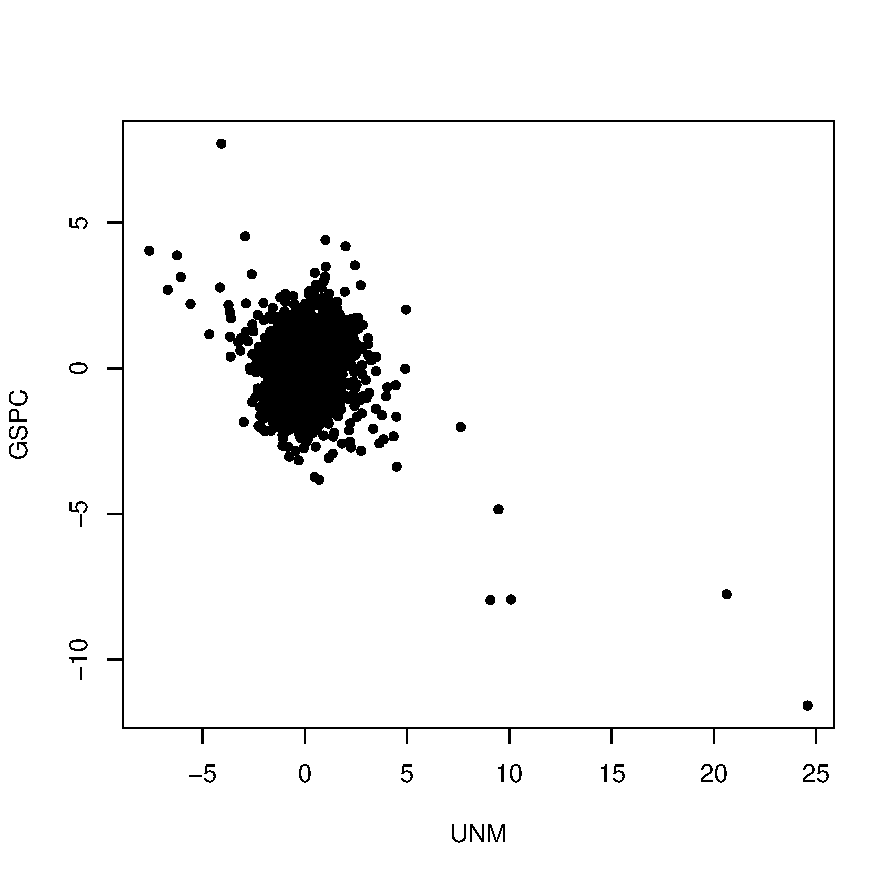
\includegraphics[width=0.4\linewidth]{scplot_UNM.pdf}}
\caption{Scatterplots of standardized innovation vectors from GARCH-DCC model for institutions AFLAC INC (AFL) and UNUMPROVIDENT CORP (UNM) with the S\&P 500 index (GSPC) as a system proxy.}
  \label{sc_dcc}
\end{figure}


\clearpage


\begin{landscape}
\section{Unconditional coverage test}
\label{uncon}

\begin{table}[H]
\tiny
\centering
\caption{Unconditional coverage tests for VaR of institutions and CoVaR at level $\pb = (0.02,0.05)$. Tail dependence models include logistic (Log),  H\"{u}sler-Reiss (HR), bilogistic (Bilog), asymmetric logistic (Alog) and that of the bivariate t distribution (t); see Supplementary Appendix~\ref{sS3} for model specifications. $E_n/e_n$ denotes the observed/nominal number of exceedances of the VaR estimate, and $E_n^b/e_n^b$ is the observed/nominal number of joint exceedances of VaR and CoVaR estimates.}
\vspace{12pt}
\begin{tabular}{cc|cccccccccccccc}
\hline
                        &           & AFL    & AIG    & ALL             & BAC             & C      & CMA    & HUM         & JPM    & LNC             & PGR    & SLM    & TRV    & UNM    & WFC    \\ \hline
\multirow{3}{*}{VaR}    & $E_n$     & 56     & 43     & 57              & 42              & 55     & 62     & 46          & 51     & 66              & 58     & 43     & 56     & 57     & 58     \\ 
                        & $e_n$     & 50.68  & 50.68  & 50.68           & 50.68           & 50.68  & 50.68  & 50.68       & 50.68  & 50.68           & 50.68  & 50.68  & 50.68  & 50.68  & 50.68  \\
                        & $p$-value & 0.4578 & 0.2633 & 0.3792          & 0.2045          & 0.5453 & 0.1205 & 0.5         & 0.9638 & \textbf{0.0377} & 0.3098 & 0.2633 & 0.4578 & 0.3792 & 0.3098 \\ \hline
\multirow{3}{*}{Log}    & $E_n^b$   & 2      & 2      & 3               & 1               & 2      & 2      & 3           & 2      & 2               & 3      & 1      & 3      & 1      & 2      \\
                        & $e_n^b$   & 2.8    & 2.15   & 2.85            & 2.1             & 2.75   & 3.1    & 2.3         & 2.55   & 3.3             & 2.9    & 2.15   & 2.8    & 2.85   & 2.9    \\
                        & $p$-value & 0.606  & 0.9155 & 0.928           & 0.3877          & 0.6265 & 0.4942 & 0.6503      & 0.7139 & 0.4297          & 0.9522 & 0.3708 & 0.9035 & 0.1965 & 0.5666 \\ \hline
\multirow{3}{*}{HR}     & $E_n^b$   & 2      & 2      & 3               & 1               & 2      & 2      & 0           & 2      & 2               & 3      & 1      & 3      & 1      & 2      \\
                        & $e_n^b$   & 2.8    & 2.15   & 2.85            & 2.1             & 2.75   & 3.1    & 2.3         & 2.55   & 3.3             & 2.9    & 2.15   & 2.8    & 2.85   & 2.9    \\
                        & $p$-value & 0.606  & 0.9155 & 0.928           & 0.3877          & 0.6265 & 0.4942 & \textbf{NA} & 0.7139 & 0.4297          & 0.9522 & 0.3708 & 0.9035 & 0.1965 & 0.5666 \\ \hline
\multirow{3}{*}{Bilog}  & $E_n^b$   & 2      & 2      & 3               & 1               & 2      & 2      & 3           & 2      & 2               & 3      & 1      & 3      & 1      & 2      \\
                        & $e_n^b$   & 2.8    & 2.15   & 2.85            & 2.1             & 2.75   & 3.1    & 2.3         & 2.55   & 3.3             & 2.9    & 2.15   & 2.8    & 2.85   & 2.9    \\
                        & $p$-value & 0.606  & 0.9155 & 0.928           & 0.3877          & 0.6265 & 0.4942 & 0.6503      & 0.7139 & 0.4297          & 0.9522 & 0.3708 & 0.9035 & 0.1965 & 0.5666 \\ \hline
\multirow{3}{*}{Alog}   & $E_n^b$   & 3      & 3      & 4               & 2               & 3      & 4      & 3           & 3      & 2               & 3      & 3      & 4      & 2      & 2      \\
                        & $e_n^b$   & 2.8    & 2.15   & 2.85            & 2.1             & 2.75   & 3.1    & 2.3         & 2.55   & 3.3             & 2.9    & 2.15   & 2.8    & 2.85   & 2.9    \\
                        & $p$-value & 0.9035 & 0.5736 & 0.5089          & 0.9431          & 0.8788 & 0.615  & 0.6503      & 0.7782 & 0.4297          & 0.9522 & 0.5736 & 0.4881 & 0.586  & 0.5666 \\ \hline
\multirow{3}{*}{t}      & $E_n^b$   & 3      & 4      & 4               & 1               & 2      & 3      & 3           & 2      & 2               & 3      & 3      & 4      & 1      & 2      \\
                        & $e_n^b$   & 2.8    & 2.15   & 2.85            & 2.1             & 2.75   & 3.1    & 2.3         & 2.55   & 3.3             & 2.9    & 2.15   & 2.8    & 2.85   & 2.9    \\
                        & $p$-value & 0.9035 & 0.245  & 0.5089          & 0.3877          & 0.6265 & 0.9533 & 0.6503      & 0.7139 & 0.4297          & 0.9522 & 0.5736 & 0.4881 & 0.1965 & 0.5666 \\ \hline
\multirow{3}{*}{FP}     & $E_n^b$   & 1      & 1      & 2               & 1               & 2      & 2      & 0           & 2      & 2               & 3      & 0      & 3      & 0      & 2      \\
                        & $e_n^b$   & 2.8    & 2.15   & 2.85            & 2.1             & 2.75   & 3.1    & 2.3         & 2.55   & 3.3             & 2.9    & 2.15   & 2.8    & 2.85   & 2.9    \\
                        & $p$-value & 0.2058  & 0.3708 & 0.5860          & 0.3877  & 0.6265 & 0.4942  & \textbf{NA}      & 0.7139 & 0.4297  & 0.9522 & \textbf{NA} & 0.9035 & \textbf{NA}  & 0.5666 \\ \hline
\multirow{3}{*}{EVT-NZ} & $E_n^b$   & 4      & 4      & 7               & 6               & 6      & 6      & 4           & 7      & 7               & 4      & 2      & 5      & 6      & 5      \\
                        & $e_n^b$   & 2.8    & 2.15   & 2.85            & 2.1             & 2.75   & 3.1    & 2.3         & 2.55   & 3.3             & 2.9    & 2.15   & 2.8    & 2.85   & 2.9    \\
                        & $p$-value & 0.4881 & 0.245  & \textbf{0.0318} & \textbf{0.0227} & 0.0798 & 0.1319 & 0.2956      & \textbf{0.0174} & 0.0672          & 0.5298 & 0.9155 & 0.2221 & 0.0931 & 0.2491 \\ \hline
\end{tabular}
\label{uncon_test}
\end{table}
\end{landscape}

\clearpage

\section{Simulation studies under model misspecification}\label{sup:Sim_Model_Misspecification}

In this section, we report results on the performance of the proposed ECQ estimator under the situation when the fitted model for the tail dependence function is misspecified. We conducted simulation studies using the settings of Section~\ref{sim}, but fit just the asymmetric logistic model for data generated using the other three tail dependence models. As summary statistics in Table~\ref{sim:summary_misspec} show, interestingly, there is both a slight lower empirical bias and a lower standard deviation when data come from the logistic and HR distributions compared to the original simulation study in which the correctly specified models were fitted. For the bivariate t distribution, there is a minor increase in bias and variance but overall results are fairly similar to those under the correct model specification. In practice, the choice of the parametric family for the tail dependence function can be based on results of comparative backtests.



\begin{table}[H]
\footnotesize
\centering
\caption{Summary statistics of ECQ estimates at level $\pb=(0.05,0.05)$ for simulation studies under model misspecification. The first row gives the true value of the ECQ under each model. }
\vspace{24pt}
\begin{tabular*}{1\textwidth}{@{\extracolsep{\fill}} c|ccc}\hline\hline
       & logistic & HR       & bivariate t      \\ \hline\hline
$Q_{Y|X}(0.05|0.05)$ & 367.31 & 399.48  & 6.81 \\  
\hline
Mean  & 389.01 & 418.78  & 6.44 \\ 
Median & 377.18 & 409.95  & 6.30 \\ 
Standard deviation     & 89.34 & 84.43 &  1.20 \\ \hline
\end{tabular*}
\label{sim:summary_misspec}
\end{table}

\begin{figure}[H]
  \centering 
  \subfigure[Logistic model]{
    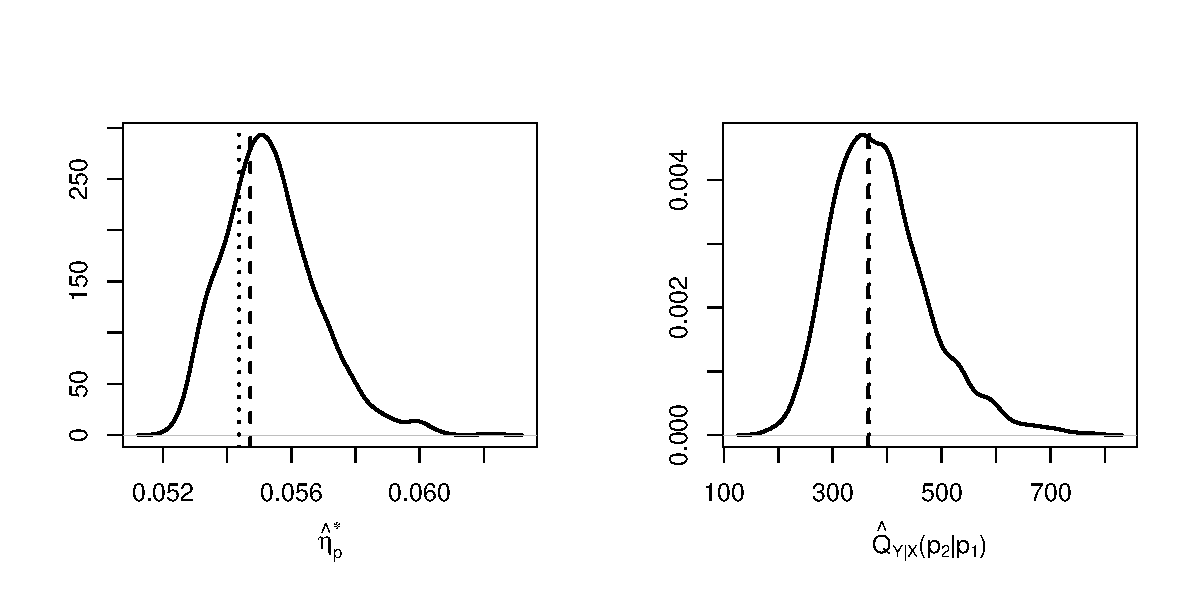
\includegraphics[width=0.6\linewidth]{log_alog.pdf}}
    \end{figure}
    \begin{figure}[H]
      \centering 
    \subfigure[HR model]{
    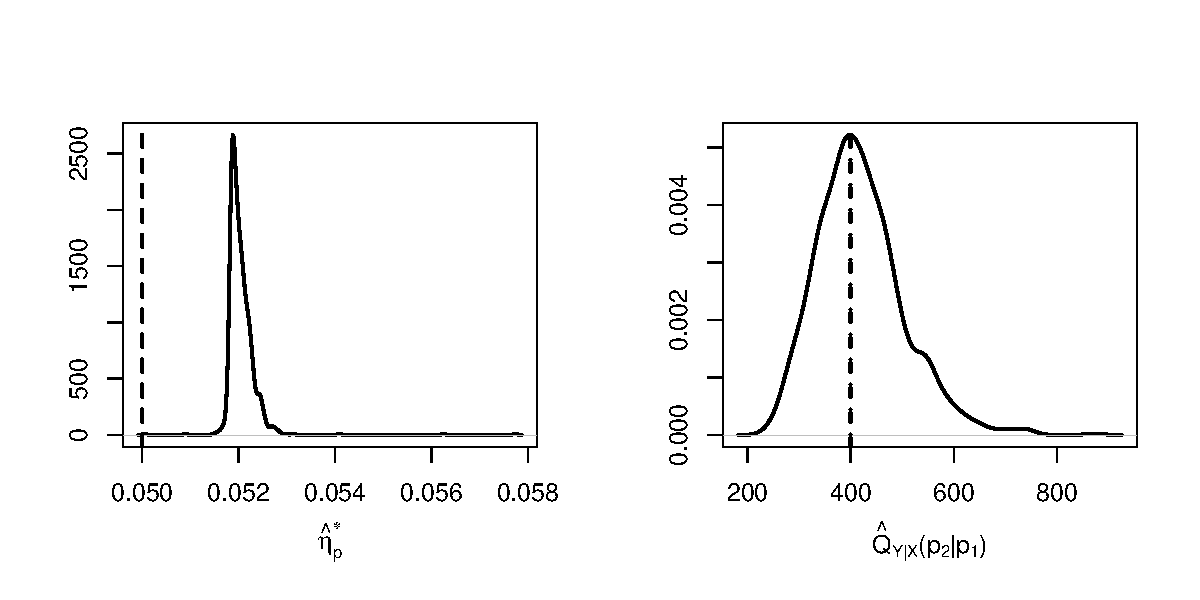
\includegraphics[width=0.6\linewidth]{hr_alog.pdf}}
    \end{figure}
    \begin{figure}[H]
          \centering 
    \subfigure[Bivariate t model]{
    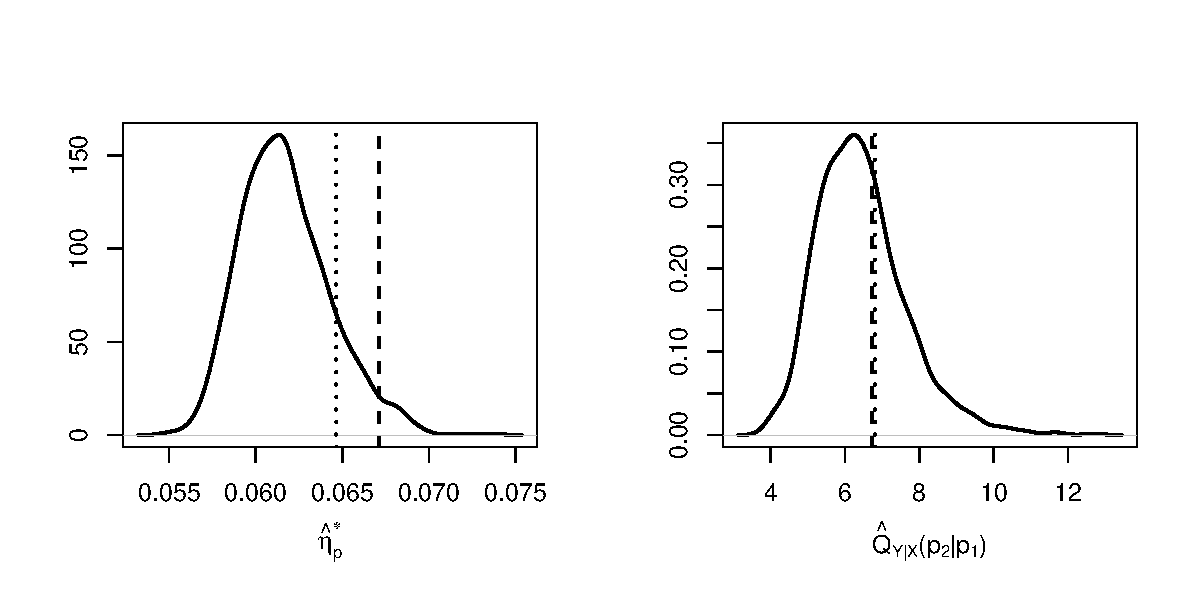
\includegraphics[width=0.6\linewidth]{t_alog.pdf}}
  \caption{The sampling densities of estimates of $\gamma$,  $\eta_p^*$, $Q_Y(p_2)$ and $Q_{Y|X}(p_2|p_1)$ for $p_1=p_2=0.05$ in the simulation study under model misspecification. The dotted vertical lines indicate true values of the quantities being estimated. The dashed vertical lines indicate the true values of $\eta_\pb$ and $Q_{Y|X}^*(p_2|p_1)$, respectively.}
  \label{sim:plot_misspec}
\end{figure}

%\clearpage

\bibliographystyle{plainnat} 

\begin{thebibliography}{29}
\providecommand{\natexlab}[1]{#1}
\providecommand{\url}[1]{\texttt{#1}}
\expandafter\ifx\csname urlstyle\endcsname\relax
  \providecommand{\doi}[1]{doi: #1}\else
  \providecommand{\doi}{doi: \begingroup \urlstyle{rm}\Url}\fi
  
\bibitem[Bollerslev(1986)]{Bollerslev1986}
T.~Bollerslev.
\newblock Generalized autoregressive conditional heteroskedasticity.
\newblock \emph{Journal of Econometrics}, 31:\penalty0 307--327, 1986.  
  
%\bibitem[de~Haan and Ferreira(2006)]{dHF2006_sup}
%L.~de~Haan and A.~Ferreira.
%\newblock \emph{Extreme Value Theory: An Introduction}.
%\newblock Springer Science \& Business Media, 2006.

\bibitem[Demarta and McNeil(2005)]{DemartaMcNeil2005}
S. Demarta and A.~J. McNeil.
\newblock The t copula and related copulas.
\newblock \emph{International Statistical Review}, 73\penalty0:\penalty0
  111--129, 2005.

%\bibitem[Einmahl et~al.(2012)Einmahl, Krajina, and Segers]{Einmahl_etal2012_sup}
%J.H. Einmahl, A.~Krajina, and J.~Segers.
%\newblock An {M}-estimator for tail dependence in arbitrary dimensions.
%\newblock \emph{The Annals of Statistics}, 40:\penalty0 1764--1793, 2012.
  
\bibitem[Fern{\'a}ndez and Steel(1998)]{FernandezSteel1998}
C.~Fern{\'a}ndez and M.~Steel.
\newblock On {B}ayesian modeling of fat tails and skewness.
\newblock \emph{Journal of the American Statistical Association}, 93:\penalty0
  359--371, 1998.
  
\bibitem[Girard et~al.(2021)Girard, Stupfler and Usseglio-Carleve]{Girard_etal2021}
S. Girard, G. Stupfler and A. Usseglio-Carleve.
\newblock Extreme conditional expectile estimation in heavy-tailed heteroscedastic regression models.
\newblock \emph{Annals of Statistics}, 49(6):\penalty0 3358–3382, 2021.

    
  
\bibitem[Girardi and Erg{\"u}n(2013)]{Girardi2013_sup}
G.~Girardi and A.T. Erg{\"u}n.
\newblock Systemic risk measurement: Multivariate {GARCH} estimation of
  {CoVaR}.
\newblock \emph{Journal of Banking \& Finance}, 37:\penalty0 3169--3180, 2013.

\bibitem[Hoga(2019)]{Hoga2019_sup}
Y. Hoga.
\newblock Confidence intervals for conditional tail risk measures in ARMA--GARCH models.
\newblock \emph{Journal of Business \& Economic Statistics}, 37(4): 613--624, 2019.

\bibitem[Hoga(2022)]{Hoga2022}
Y. Hoga.
\newblock Limit theory for forecasts of extreme distortion risk measures and expectiles.
\newblock \emph{Journal of Financial Econometrics}, 20(1): 18–44, 2022.


\bibitem[Nolde and Zhang(2020)]{NoldeZhang2018_sup}
N.~Nolde and J.~Zhang.
\newblock Conditional extremes in asymmetric financial markets.
\newblock \emph{Journal of Business \& Economic Statistics}, 38: 201--213, 2020.

\end{thebibliography}

%\end{appendices}